\chapter{Xây dựng ứng dụng}
Để hiển thị kết quả của mô hình một cách trực quan thì nhóm đã xây dựng một ứng dụng hiển thị trên website cho phép người dùng upload dữ liệu, sau đó hiển thị kết quả phân đoạn và mô hình 3D. Phần này sẽ trình bày về cấu trúc, luồng xử lý, cách xây dựng và các chức năng chính của ứng dụng.
\section{Cấu trúc ứng dụng}
Ứng dụng được xây dựng theo mô hình client - server API (gồm hai phần là client và server riêng biệt hoạt động với nhau qua cơ chế gọi API).
\begin{figure}[h]
\centering
    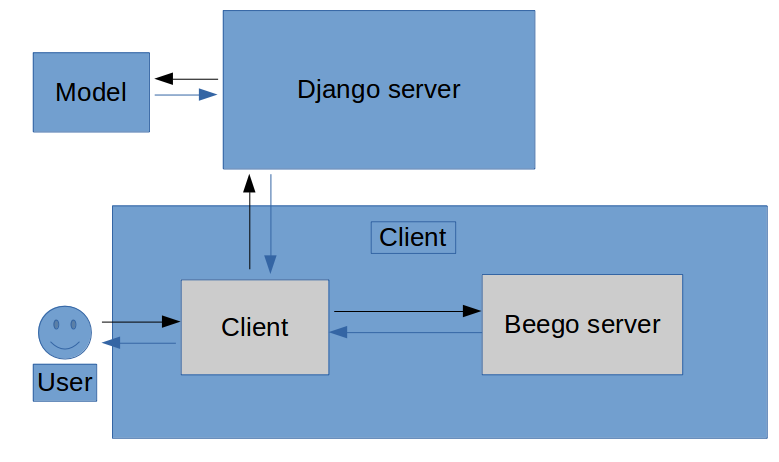
\includegraphics[totalheight=7cm]{Images/app_struct.png}
    \caption{Cấu trúc chính của ứng dụng}
    \label{skip_conn}
\end{figure}
\section{RESTful API}
REST (Representational State Transfer) ra đời vào năm 2000 bởi Roy Thomas Fielding. Ta có thể gọi đây là các ràng buộc và quy ước mà khi hệ thống nào làm theo thì được gọi là REST.\\
API (Application Programming Interface) là phương thức để kết nối các thư viện và ứng dụng với nhau \cite{website:api}.\\

RESTful API là một tiêu chuẩn dùng trong việc thết kế các thiết kế API cho các ứng dụng web để quản lý các tài nguyên. RESTful là một trong những kiểu thiết kế API được sử dụng phổ biến nhất ngày nay \cite{website:restfulapi}.\\
Về cơ bản thì RESTful API là một khái niệm khá trừu tượng nhưng lại rất dễ sử dụng. Để cho dễ hiểu thì phần này sẽ trình bày về cấu trúc và cách sử dụng, đồng thời gọi tắt là ``API`` cho cơ chế này.\\
Cấu trúc của một RESTful API gồm những phần như sau:
\begin{itemize}
    \item METHOD (bắt buộc): Gồm các phương thức cơ bản như GET, POST, PUT, DELETE.
    \item URL (bắt buộc): đường dẫn của API(đường dẫn này sẽ được phân chia trong Routers bên phía server).
    \item DATA (tùy chọn): đối tượng JSON mô tả dữ liệu kèm theo gửi lên server.
    \item HEADER (tùy chọn): Đối tượng JSON thường dùng trong việc bảo mật và xác thực người dùng.
    \item PARAM (tùy chọn): Các tham số đi kèm sau dấu ``?`` của URL.
\end{itemize}
Các bước gọi và phản hồi API cơ bản như sau:
Phía client tạo một API chứa những thông tin cần thiết như trên, phía server sẽ kiểm tra header có phù hợp hay không, sau đó nhận dữ liệu, kiểm tra tính hợp lệ của dữ liệu, xử lý và trả lại dữ liệu cần thiết cho client nếu có.
\begin{figure}[h]
\centering
    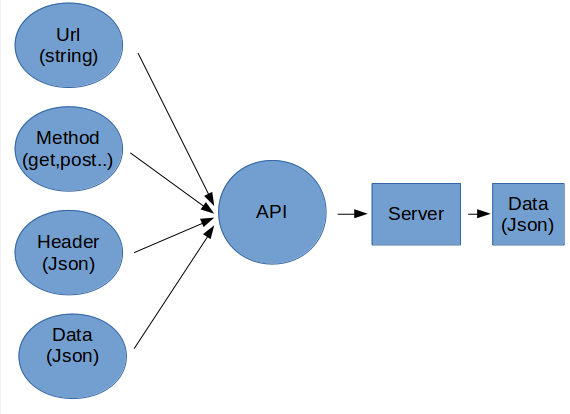
\includegraphics[totalheight=7cm]{Images/app_json.png}
    \caption{Cấu trúc và luồng xử lý của một API}
    \label{skip_conn}
\end{figure}
\section{Các ngôn ngữ, framework và các thư viện liên quan}
Phần này sẽ trình bày sơ qua về các ngôn ngữ lập trình, các framework và các thư viện liên quan được sử dụng để xây dựng ứng dụng.
\subsection{Ngôn ngữ Python}
Python là một ngôn ngữ bậc cao, mã nguồn mở ra mắt lần đầu vào năm 1991 bởi Guido van Rossum. Hiện tại thì nó có hai phiên bản phổ biến là Python 2 và Python 3(trong ứng dụng sử dụng Python 3 bản 3.5.2).\\
Một số ưu điểm của Python như sau:
\begin{itemize}
    \item Cú pháp đơn giản, cấu trúc rõ ràng, dễ đọc dễ học nên code ngắn gọn nhưng đem lại hiệu quả cao.
    \item Có rất nhiều thư viện và framework hỗ trợ đặc biệt trong việc xây dựng các ứng dụng về học máy, đồng thời cộng đồng hỗ trợ rất nhiều nên dễ dàng được hỗ trợ khi gặp khó khăn.
    \item Dễ dàng kết hợp với các ngôn ngữ khác.
\end{itemize}
Với những ưu điểm nêu trên, Python được sử dụng khá rộng rãi trong việc lập trình game, website và đặc biệt là lập trình các hệ thống học máy đang hot hiện nay.\\

Để biết thêm về Python có thể tham khảo tại \href{https://docs.python.org}{đây}.
\subsection{Framework Django}
Django là framework phổ biến nhất của Python và được viết hoàn toàn bằng Python, ra đời vào năm 2005 bởi Adrian Holovaty và Simon Willison. Django chủ yếu được sử dụng để xây dựng các ứng dụng website theo mô hình Model-View-Template (MVT) với ngôn ngữ xử lý phía server là Python. Django server cung cấp cơ chế phục vụ API cho các client gọi vào. Phần ứng dụng của nhóm chỉ sử dụng tới cơ chế này nên sẽ không trình bày nhiều về framework Django. Để biết thêm về framework Django có thể tham khảo tại \href{https://docs.djangoproject.com/en/2.2/}{đây}. 
\subsection{Các thư viện hỗ trợ trong Python}
Để cho việc lập trình được nhanh chóng thì ứng dụng sử dụng rất nhiều các thư viện của Python, đặc biệt có thể kế đến như:
\begin{itemize}
    \item zipfile: hỗ trợ việc nén/giải nén file.
    \item SimpleITK: hỗ trợ việc đọc file dạng raw/mhd nhanh chóng.
    \item numpy: hỗ trợ việc tính toán nhanh chóng, đặc biệt trên các mảng nhiều chiều.
    \item csv: hỗ trợ đọc và ghi file csv.
    \item skimage: cung cấp module measure để tạo tập đỉnh và mặt từ mảng ba chiều.
\end{itemize}
\subsection{Ngôn ngữ Golang}
Golang hay còn được gọi là Go được thiết kế và phát triển bởi Robert Griesemer, Rob Pike và Ken Thompson tại Google vào năm 2007, được giới thiệu vào năm 2009 và hiện tại được sử dụng trong hầu hết trong các sản phẩm của Google. Hiện tại thì Go khá được ưa chuộng bởi các đặc điểm sau \cite{website:golang}:
\begin{itemize}
    \item Hỗ trợ khai báo kiểu dữ liệu động.
    \item Tốc độ biên dịch nhanh.
    \item Hỗ trợ các tác vụ đồng thời.
    \item Ngôn ngữ đơn giản, ngắn gọn.
\end{itemize}
Nói tóm lại, Go có tốc độ xử lý nhanh tương đương như C/C++ nhưng cấu trúc đơn giản và hỗ trợ trình dọn rác tự động nên dễ sử dụng, hiệu quả cao. Để biết thêm thông tin về Go thì có thể tham khảo tại \href{https://golang.org/doc/}{đây}. 
\subsection{Framework Beego}
Beego là một framework mã nguồn mở cho cộng đồng sử dụng miễn phí và phát triển nó theo đường dẫn \href{https://github.com/astaxie/beego}{này}.\\
Ta sử dụng Beego để tạo một ứng dụng web chạy trực tiếp trên máy chủ local. Khi cài đặt và tạo một dự án bằng Beego, ta sẽ có một cây thư mục hoàn chỉnh cho các thành phần chính của ứng dụng.\\
\begin{figure}[h]
\centering
    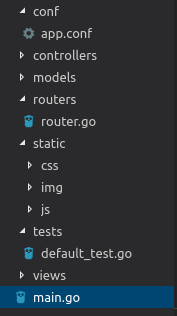
\includegraphics[totalheight=7cm]{Images/app_beego_struct_folder.png}
    \caption{Cây thư mục làm việc trong Beego}
    \label{skip_conn}
\end{figure}
Ứng dụng web được tạo bởi Beego theo mô hình Model-View-Controller (MVC) và giao tiếp qua cơ chế gọi API, các thành phần của ứng dụng được giải thích ngắn gọn như sau:
\begin{itemize}
    \item Conf: chứa file config định nghĩa một số thông tin chính như cổng, tên, thông tin cơ sở dữ liệu…
    \item Controllers: Nhận và xử lý dữ liệu từ bên ngoài, rồi gọi tới Model và gửi dữ liệu ra nếu có.
    \item Main.go: File để chạy ứng dụng.
    \item Models: Nhận dữ liệu đã hợp lệ từ Controllers để xử lý, thường là các tác vụ liên quan tới cơ sở dữ liệu và trả về dữ liệu cần thiết cho Controller.
    \item Routers: Quản lý, phân chia các API cho các Controller tương ứng.
    \item Static: chứa các dữ liệu cần thiết cho phía client.
    \item Tests: Dùng để kiểm tra lại ứng dụng, là nơi làm việc của kiểm tra viên.
    \item Views: Mặc định chứa file hiển thị trang chủ.
\end{itemize}
Để tìm hiểu kĩ hơn về framework Beego có thể tham khảo tại \href{ https://beego.me/docs}{đây}.

\subsection{Framework AngularJS}
AngularJS có thể gọi là một framework được viết bằng Javascript. AngularJS đưa ra hướng dẫn cụ thể trên mã lệnh HTML với các tiền tố ``ng-`` hay còn được gọi là directives \cite{website:angularjs}.\\
Để sử dụng thì chỉ cần nhúng đường dẫn tới file angular.min.js như sử dụng các thư viện của Javascript.\\
Một số directive quan trọng có thể kể đến như sau:
\begin{itemize}
    \item ng-app: Đánh dấu thẻ HTML mà AngularJS được bắt đầu sử dụng.
    \item ng-model: giá trị HTML trong thẻ này tương đương với biến \$scope trong phần Controller tương ứng.
    \item ng-change, ng-click: bắt sự kiện thay đổi, click để gọi hàm \$scope tương ứng.
\end{itemize}
Một điều quan trọng nữa là AngularJS hỗ trợ gọi API để gửi và nhận dữ liệu một cách dễ dàng qua biến \$http.
Để biết thêm về AngularJS có thể tham khảo tại \href{ https://docs.angularjs.org/api/ng/service/\$document
}{đây}.
\subsection{Một số thư viện khác hỗ trợ phần hiển thị}
Ngoài những thư viện và framework quan trọng kể trên thì ứng dụng của nhóm sử dụng khá nhiều các thư viện hỗ trợ phần thiết kế giao diện như:
\begin{itemize}
    \item Bootstrap: Thư viện quen thuộc để xây dựng giao diện responsive dễ dàng. Trong ứng dụng này sử dụng bootstrap phiên bản 3.3.7.
    \item Plotly: Thư viện giúp hiển thị hình ảnh 3D từ file csv chứa tập đỉnh và mặt.
    \item Jquery, Font Awesome, Rangesslider: hỗ trợ việc hiển thị được tốt và hiệu quả hơn.
\end{itemize}
\section{Xây dựng phần Django server}
Phần server chính của ứng dụng (Django server) được xây dựng bằng ngôn ngữ Python với framework là Django, làm việc trực tiếp với mô hình đã huấn luyện được và server này sẽ cung cấp một API để client gọi vào. 
\begin{figure}[h]
\centering
    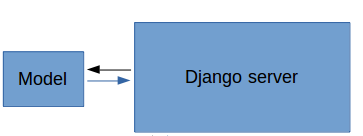
\includegraphics[totalheight=5cm]{Images/app_posdjangoserver.png}
    \caption{Vị trí Django server trong cấu trúc ứng dụng}
    \label{skip_conn}
\end{figure}
Luồng xử lý phần server này được chia làm các giai đoạn như sau: 
\begin{itemize}
    \item Quá trình xử lý dữ liệu đầu vào và chạy model.
    \item Quá trình xử lý sau chạy model.
    \item Tạo đối tượng JSON và gửi cho client.
\end{itemize}
\begin{figure}[h]
\centering
    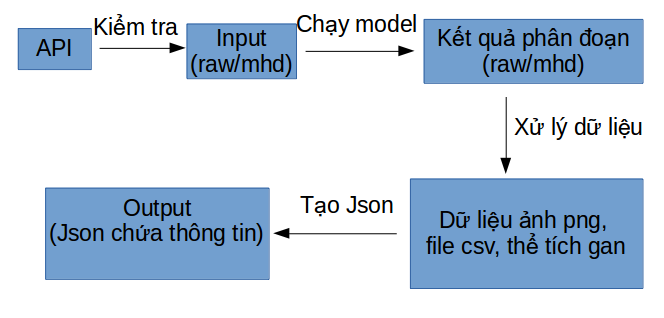
\includegraphics[totalheight=7cm]{Images/app_django_struct.png}
    \caption{Luồng xử lý trong Django server}
    \label{skip_conn}
\end{figure}
\subsection{Quá trình xử lý dữ liệu đầu vào và chạy model}
Dữ liệu đầu vào để server xử lý phải là dữ liệu có định dạng raw/mhd (định dạng như tập Sliver07). Dữ liệu có thể chỉ cần tập ảnh scan nếu muốn phân đoạn hoặc bao gồm cả tập nhãn nếu muốn so sánh và đánh giá kết quả phân đoạn.\\
Sau khi nhận dữ liệu đầu vào dưới dạng API, server sẽ tiến hành kiểm tra API này, sau đó lấy dữ liệu và lưu lại, chạy model để cho ra kết quả phân đoạn. Đầu ra của quá trình này cũng là file có định dạng raw/mhd. Thời gian chạy cho quá trình này mất khá nhiều thời gian khi chạy trên máy local không có GPU.
\begin{figure}[h]
\centering
    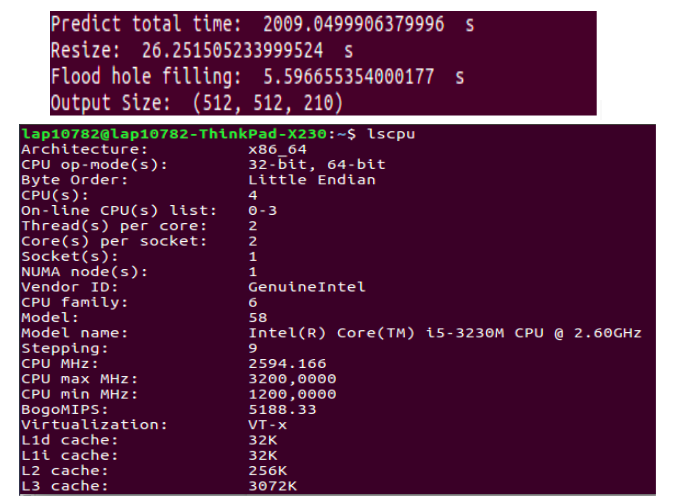
\includegraphics[totalheight=7cm]{Images/app_configuration.png}
    \caption{Thời gian chạy model với cấu hình máy tương ứng}
    \label{skip_conn}
\end{figure}
\subsection{Quá trình xử lý sau chạy model}
Khi chạy xong model, sử dụng các thư viện hỗ trợ của Python để xử lý dữ liệu như sau:
\begin{itemize}
    \item Thư viện SimpleITK đọc hình ảnh dạng raw/mhd ra các thông tin cần thiết như mảng chứa nội dung các hình ảnh, spacing của dữ liệu, từ đó tính thể tích một cách dễ dàng.
    \item Thư viện numpy xử lý các mảng dữ liệu để ra các hình ảnh dạng so sánh, dán kết quả lên scan.
    \item Module measure trong thư viện skimage tạo tập đỉnh và mặt từ mảng hình ảnh phân đoạn, sau đó dùng thư viện csv để đọc và ghi các tập đỉnh và mặt này vào file.
\end{itemize}
Tất các các hình ảnh đầu ra của quá trình này đều có định dạng là png. Sau khi tạo các thông tin đó thì tạo file zip kèm theo cho mỗi tập. Các tập dữ liệu tạo ra tương ứng như sau:
\begin{itemize}
    \item Với tập đầu vào chỉ có scan, kết quả của quá trình này sẽ bao gồm: Tập ảnh scan, tập ảnh kết quả phân đoạn, tập ảnh phân đoạn dán lên scan, file csv gồm thông tin tập đỉnh và mặt của mô hình gan 3D, thể tích gan theo kết quả phân đoạn.
    \item Với tập có cả scan và nhãn thì kết quả bao gồm: Tập ảnh scan, tập ảnh nhãn, tập ảnh kết quả phân đoạn so sánh với nhãn,  tập ảnh kết quả phân đoạn so sánh với nhãn dán lên scan, file csv gồm thông tin tập đỉnh và mặt mô hình gan 3D và thể tích gan của kết quả phân đoạn và của nhãn.
\end{itemize}


\begin{figure}[h]
\centering
    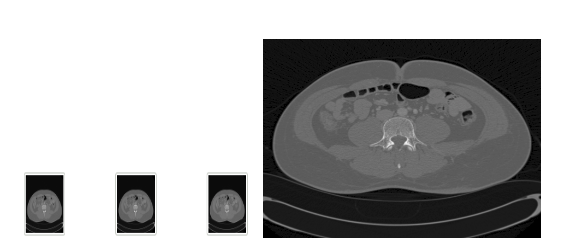
\includegraphics[totalheight=7cm]{Images/app_listscan.png}
    \caption{Tập ảnh scan được lưu lại}
    \label{skip_conn}
\end{figure}


\begin{figure}[h]
\centering
    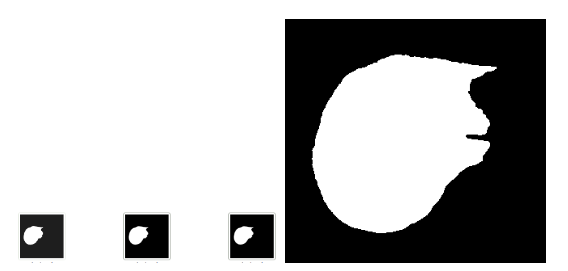
\includegraphics[totalheight=7cm]{Images/app_listlabel.png}
    \caption{Tập ảnh phân đoạn/nhãn được lưu lại}
    \label{skip_conn}
\end{figure}

\begin{figure}[h]
\centering
    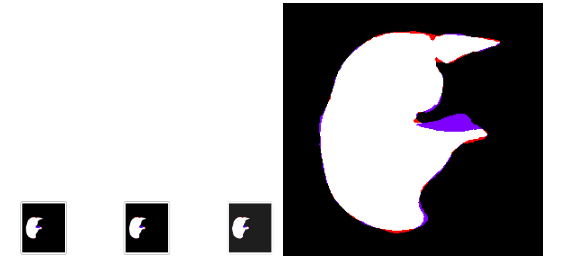
\includegraphics[totalheight=7cm]{Images/app_listcompare.png}
    \caption{Tập ảnh phân đoạn so sánh với nhãn được lưu lại(nếu có nhãn)}
    \label{skip_conn}
\end{figure}


\begin{figure}[h]
\centering
    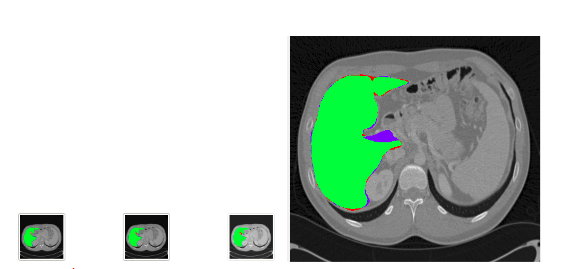
\includegraphics[totalheight=7cm]{Images/app_listoverlap.png}
    \caption{Tập ảnh kết quả dán lên scan}
    \label{skip_conn}
\end{figure}

\subsection{Tạo đối tượng JSON và gửi cho client}
Với cơ chế gọi API, dữ liệu nhận và gửi sẽ ở định dạng JSON nên dữ liệu trả về cho client sẽ là một đối tượng JSON với các trường dữ liệu được mô tả như sau (các đường dẫn tương ứng là các file đã được lưu trong server):
\begin{itemize}
    \item ListPredict: mảng các đường dẫn của ảnh kết quả phân đoạn.
    \item ListLabel: mảng các đường dẫn của ảnh nhãn(nếu có).
    \item ListOverlap: mảng các đường dẫn ảnh kết quả dán lên scan.
    \item CsvFileLabel: đường dẫn tới file csv của nhãn(nếu có).
    \item CsvFilePredict: đường dẫn tới file csv kết quả phân đoạn.
    \item LinkZip: đối tượng json chứa các đường dẫn tới file zip của các tập.
    \item VolumePredict: thông tin thể tích theo kết quả phân đoạn.
    \item VolumePredict: thông tin thể tích theo kết quả phân đoạn.
\end{itemize}
Sau khi tạo xong đối tượng json sẽ được gửi về client xử lý.

\section{Xây dựng phần client}
Với cấu trúc server như trên chúng ta có thể xây dựng phần client một cách linh động sao cho trực quan nhất trên bất cứ nền tảng nào qua cơ chế API. Ở phần này thì nhóm xây dựng phần client này trên nền tảng website sử dụng framework Beego, với ngôn ngữ phía server là Golang, phía client là HTML, CSS, Javascript cho giao diện, sử dụng framework AngularJS để giao tiếp với phía server Golang.
\begin{figure}[h]
\centering
    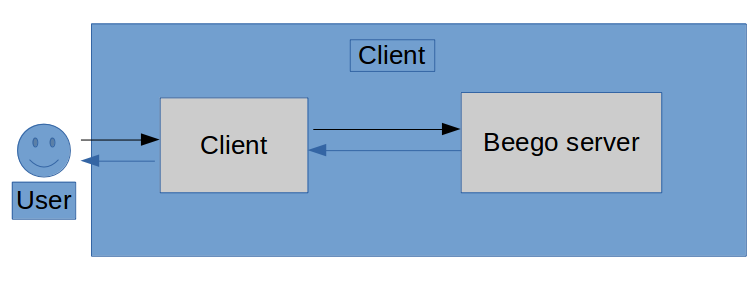
\includegraphics[totalheight=5cm]{Images/app_postclient.png}
    \caption{Vị trí phần client trong cấu trúc ứng dụng}
    \label{skip_conn}
\end{figure}
Các công việc chính theo thứ tự của phần client này như sau:
\begin{itemize}
    \item Upload dữ liệu và lấy đường dẫn cần thiết từ Django server.
    \item Beego server thực hiện việc tải về, giải nén các file từ đường dẫn.
    \item Beego server tạo đối tượng JSON để gửi lại cho giao diện hiển thị.
\end{itemize}

\begin{figure}[h]
\centering
    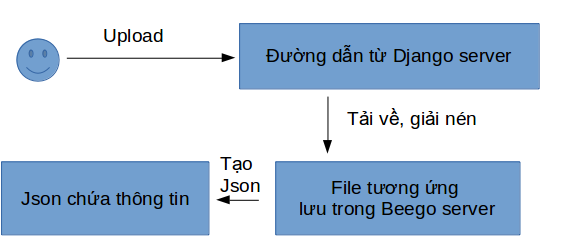
\includegraphics[totalheight=7cm]{Images/app_beego_struct.png}
    \caption{Luồng xử lý phần client chính}
    \label{skip_conn}
\end{figure}

\paragraph{Upload dữ liệu:} Khi upload dữ liệu dạng file zip, phía client Javascript phải tạo dữ liệu để gọi API lên Django server. Dữ liệu này là một đối tượng JSON không giống thông thường mà nó phải khai báo kiểu FormData() mới lưu trữ được nội dung file mà người dùng upload qua thẻ input.\\
\paragraph{Công việc của Beego server:} Ngoài việc tạo đường dẫn trên máy chủ, Beego sẽ nhận các đường dẫn các file trong Django server từ client qua API, sau đó thực hiện việc giải nén và tạo file lưu trữ nội dung của lần phân đoạn sau cùng. Sau đó tạo đối tượng JSON để gửi lại dữ liệu cho client qua việc phản hồi API.
\paragraph{Hiển thị mô hình 3D:} Như đã nêu ở trên, việc hiển thị mô hình 3D của lá gan sẽ dùng tới thư viện Plotly. Chỉ cần nhúng file plotly.js vào, ta có thể đọc file csv chứa tập đỉnh và mặt do Django server đã tạo, sau đó tạo một đối tượng JSON chứa các tập đỉnh và mặt này và tiếp tục dùng Plotly để đọc đối tượng JSON và tạo ra mô hình 3D với kiểu hiển thị là "mesh3D".

\begin{figure}[h]
\centering
    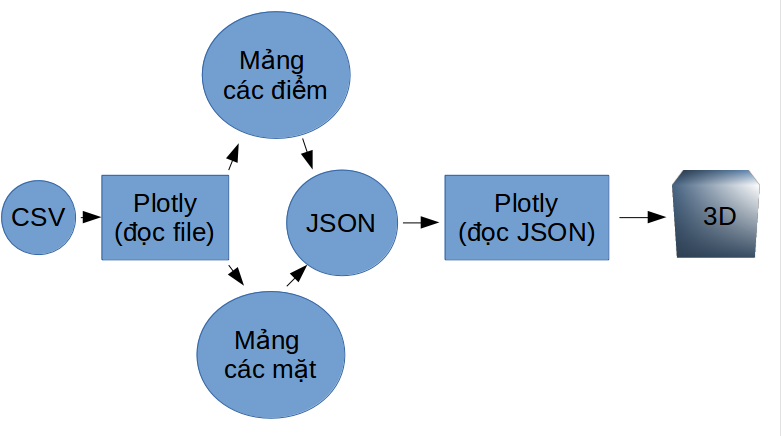
\includegraphics[totalheight=7cm]{Images/app_show3d.png}
    \caption{Luồng xử lý việc hiển thị mô hình 3D bằng Plotly}
    \label{skip_conn}
\end{figure}

\section{Các chức năng và kết quả hiển thị của ứng dụng}
Về phần hiển thị, trang web được xây dựng khá đơn giản nhưng đảm bảo được những thông tin cần thiết của kết quả phân đoạn một lá gan.
\subsection{Trang giới thiệu}
Trang này chỉ đơn giản là giới thiệu về chức năng của website.
\begin{figure}[h]
\centering
    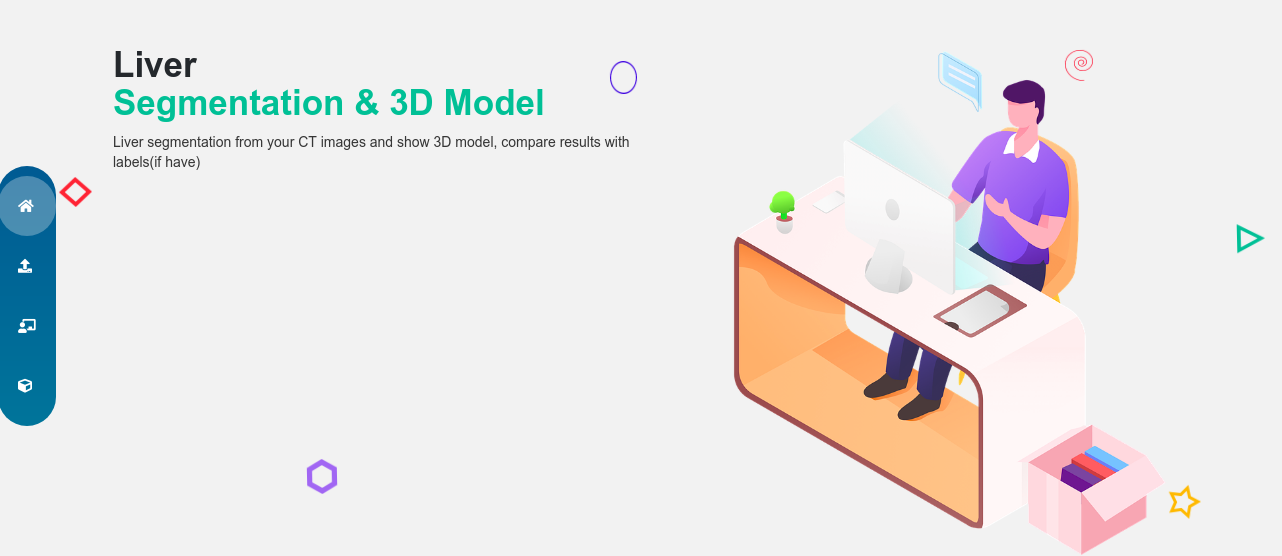
\includegraphics[totalheight=7cm]{Images/app_intro.png}
    \caption{Giao diện trang giới thiệu ứng dụng}
    \label{skip_conn}
\end{figure}
\subsection{Trang upload dữ liệu}
Trang này cho phép người dùng upload dữ liệu lên. Dữ liệu là tập scan có định dạng raw/mhd được nén trực tiếp ở dạng zip. Sau khi upload thì đợi kết quả trả về (chạy trên máy local mất khoảng 30 phút). Nếu dữ liệu có thêm nhãn thì kết quả trả về có dạng để so sánh. Kết quả sẽ được hiển thị ở trang tiếp theo.
\begin{figure}[h]
\centering
    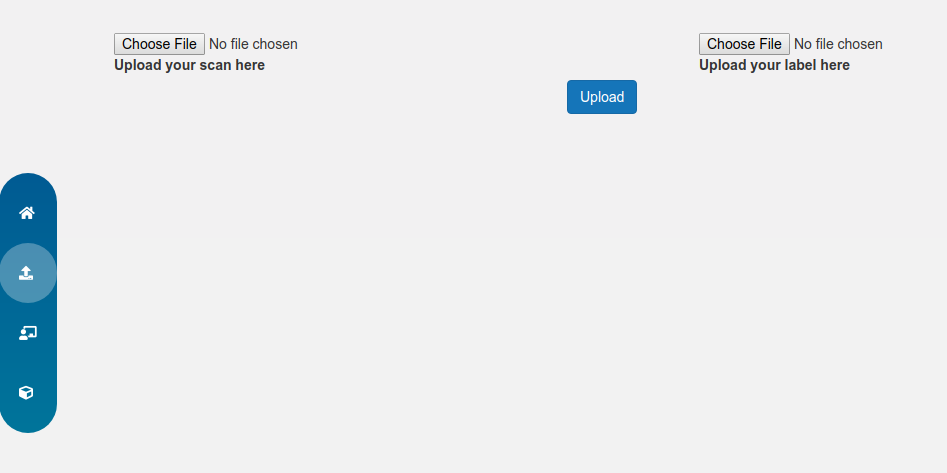
\includegraphics[totalheight=7cm]{Images/app_upload.png}
    \caption{Giao diện trang upload dữ liệu}
    \label{skip_conn}
\end{figure}
\subsection{Trang hiển thị kết quả phân đoạn}
Như đã nêu trên, nếu dữ liệu upload chỉ có scan, thì trang này hiển thị 3 mục như sau:
\begin{itemize}
    \item Ảnh scan(ảnh gốc lúc upload).
    \item Ảnh phân đoạn gan.
    \item Ảnh phân đoạn dán lên scan tương ứng.
\end{itemize}

\begin{figure}[h]
\centering
    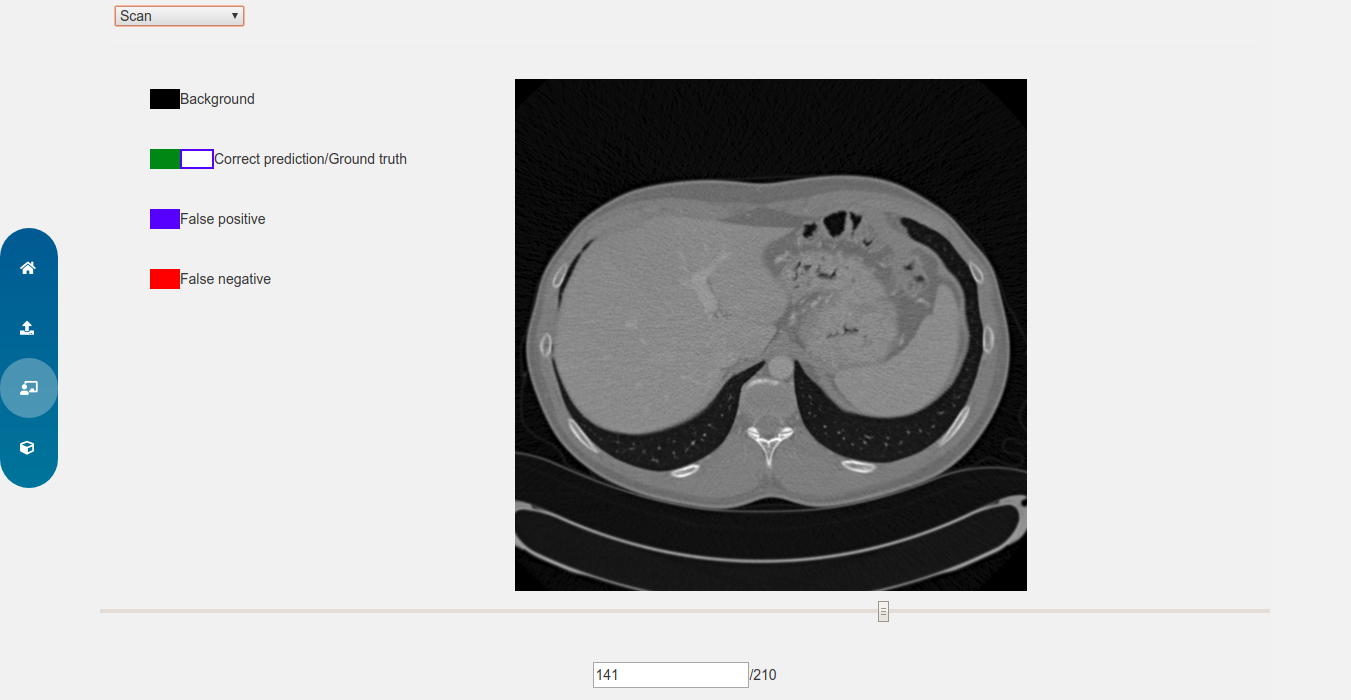
\includegraphics[totalheight=7cm]{Images/app_scan.png}
    \caption{Hiển thị ảnh scan}
    \label{skip_conn}
\end{figure}
\begin{figure}[h]
\centering
    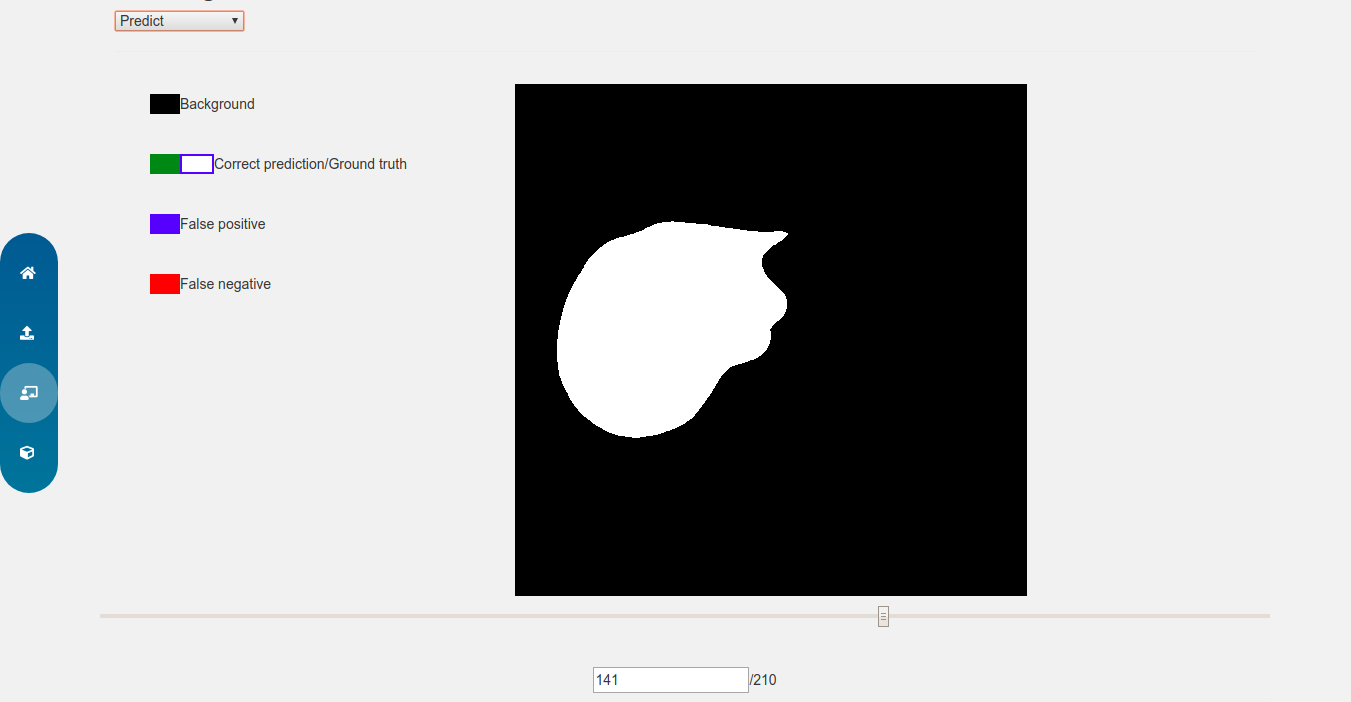
\includegraphics[totalheight=7cm]{Images/app_label.png}
    \caption{Hiển thị ảnh phân đoạn khi không có nhãn}
    \label{skip_conn}
\end{figure}
\begin{figure}[h]
\centering
    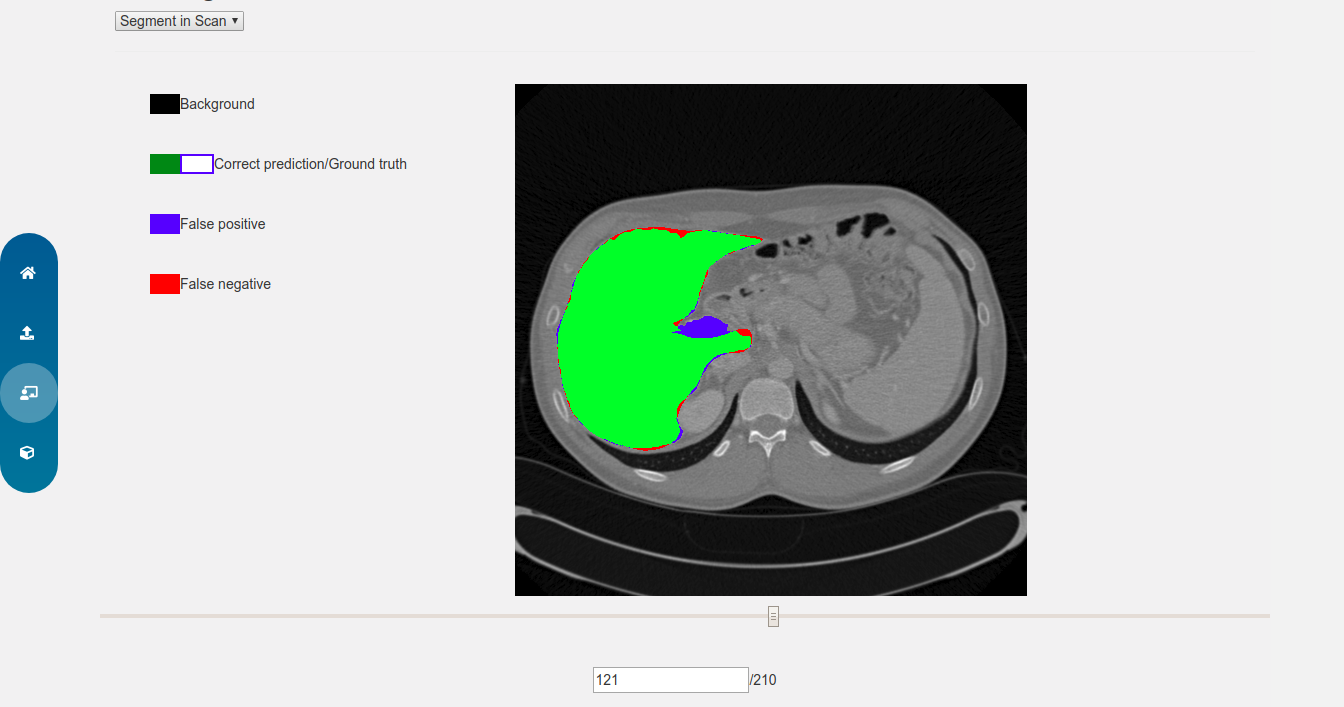
\includegraphics[totalheight=7cm]{Images/app_overlap_1.png}
    \caption{Hiển thị ảnh phân đoạn dán lên scan}
    \label{skip_conn}
\end{figure}
Nếu tập dữ liệu có thêm nhãn thì kết quả hiển thị có ảnh scan giống với mục trên, các ảnh còn lại sẽ là kết quả để so sánh với nhãn.
\begin{figure}[h]
\centering
    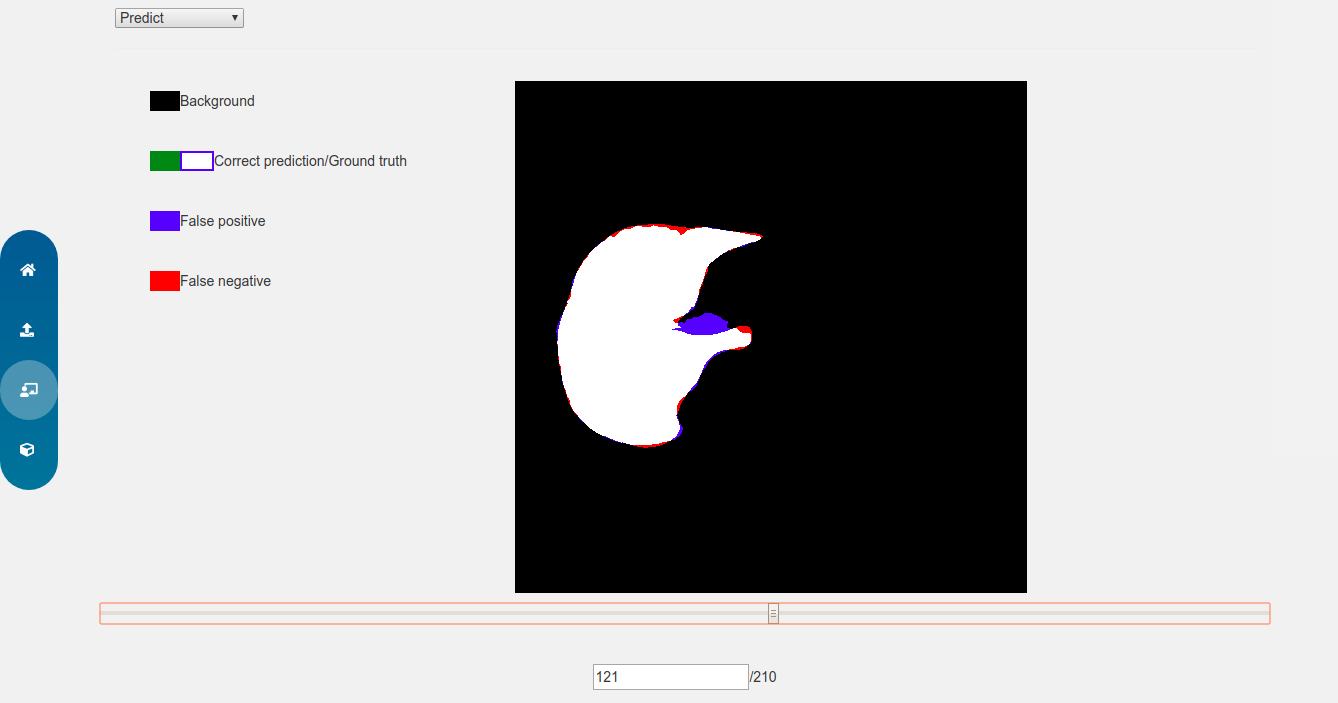
\includegraphics[totalheight=7cm]{Images/app_showscanompare.png}
    \caption{Hiển thị ảnh phân đoạn so sánh với nhãn}
    \label{skip_conn}
\end{figure}
\begin{figure}[h]
\centering
    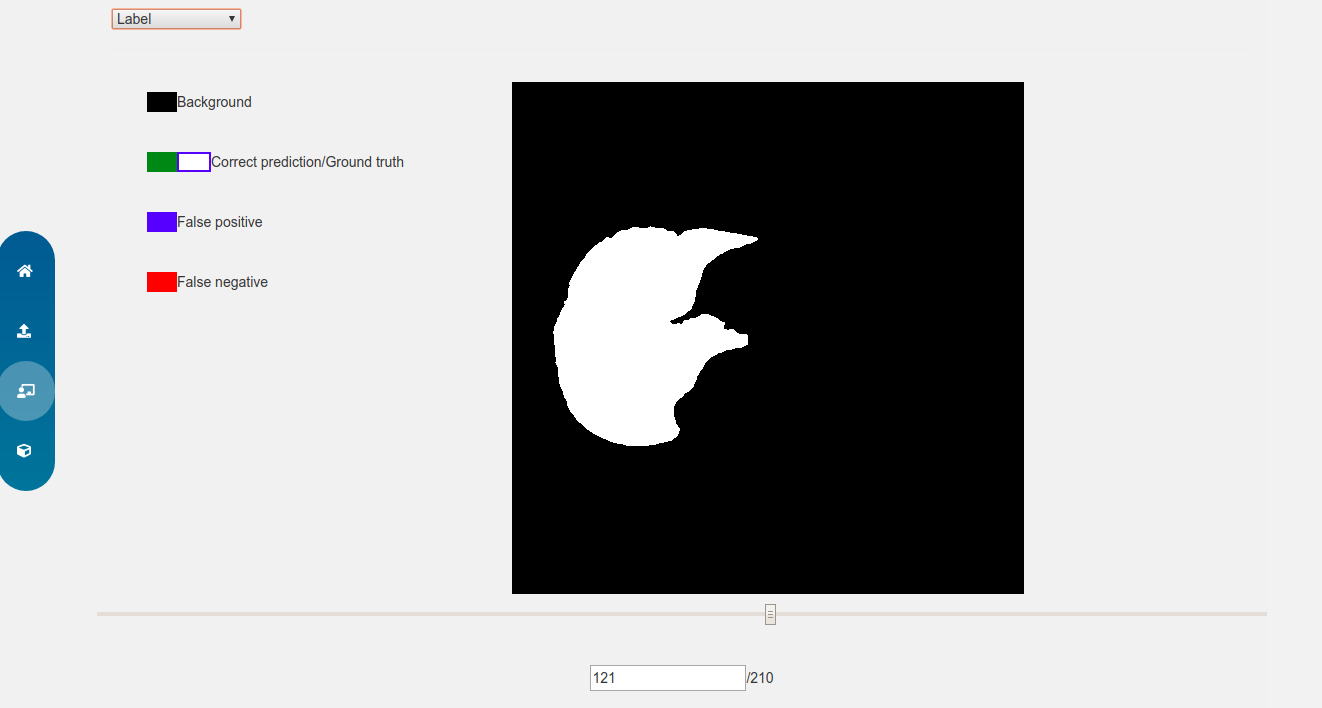
\includegraphics[totalheight=7cm]{Images/app_labelreal.png}
    \caption{Hiển thị ảnh nhãn}
    \label{skip_conn}
\end{figure}
\begin{figure}[h]
\centering
    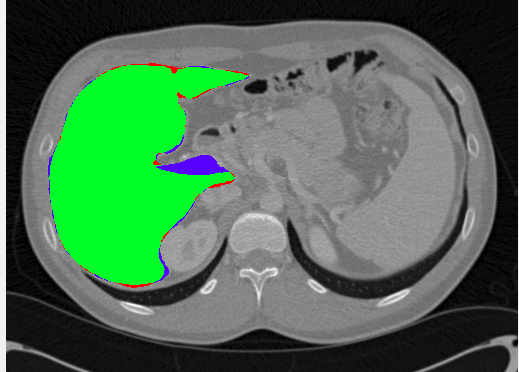
\includegraphics[totalheight=7cm]{Images/app_overlap_2.png}
    \caption{Hiển thị ảnh phân đoạn so sánh với nhãn dán lên scan}
    \label{skip_conn}
\end{figure}

\subsection{Trang hiển thị mô hình 3D}
Trang này hiển thị mô hình 3D bằng cách dùng thư viện plotly.js đọc file csv được tạo ra trong Django server đồng thời hiển thị thể tích của gan. Người dùng có thể dùng chuột để xoay, thu nhỏ, phóng to để xem chi tiết mô hình.
\begin{figure}[h]
\centering
    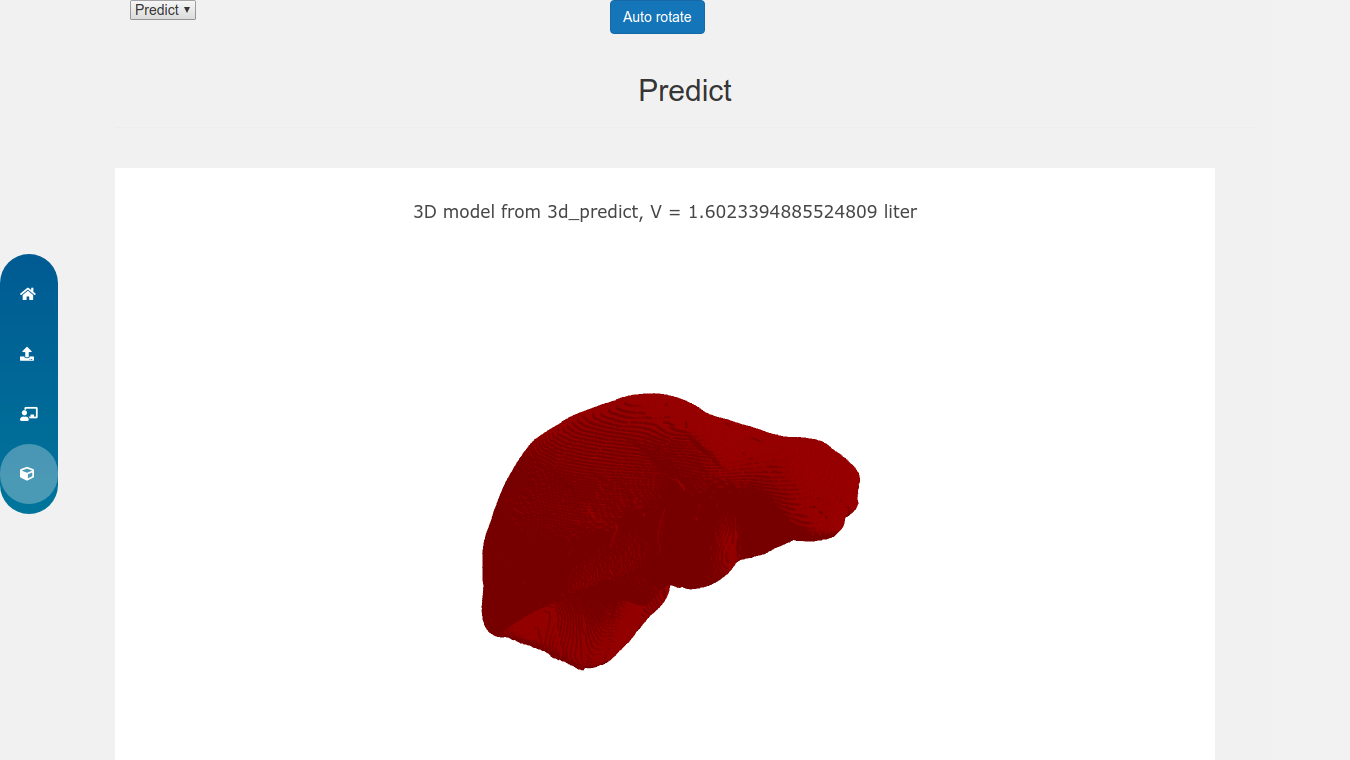
\includegraphics[totalheight=7cm]{Images/app_3dpredict.png}
    \caption{Hiển thị mô hình 3D dự đoán kèm thể tích}
    \label{skip_conn}
\end{figure}
\begin{figure}[h]
\centering
    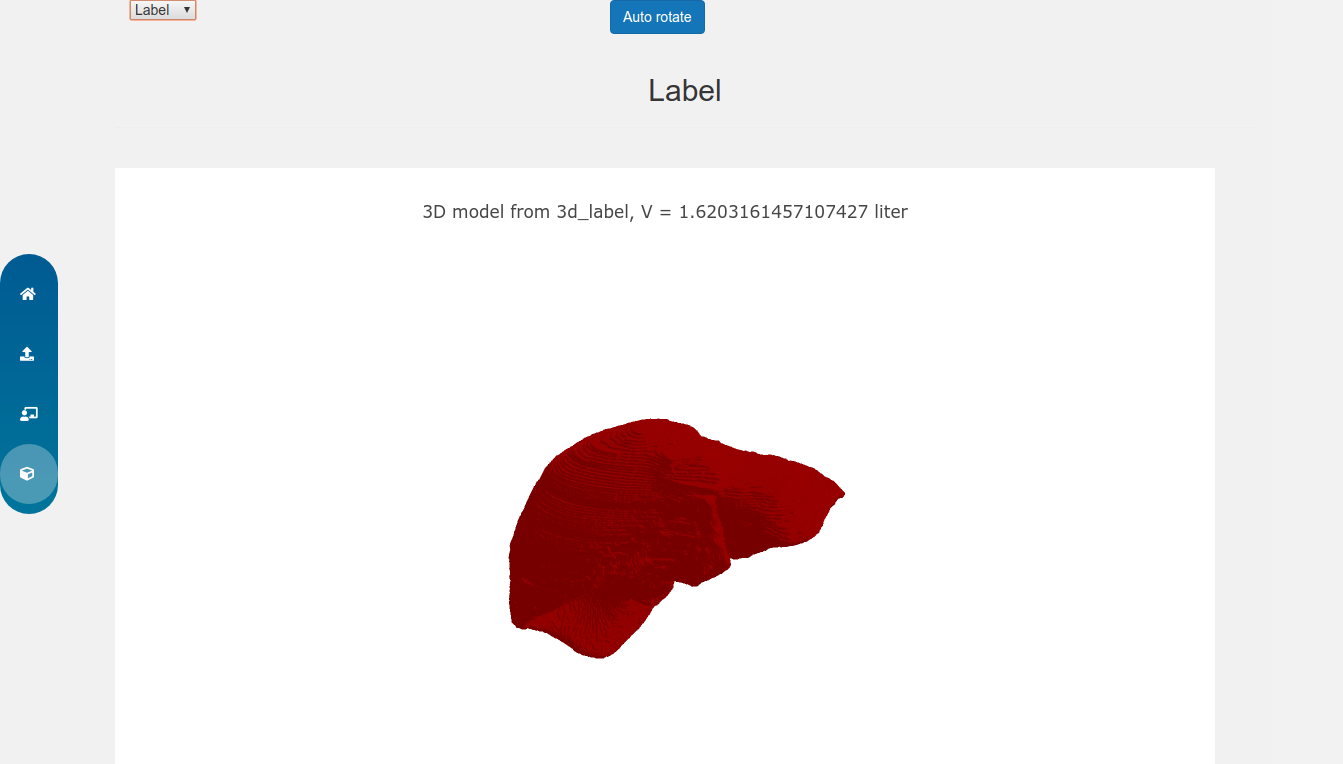
\includegraphics[totalheight=7cm]{Images/app_3dlabel.png}
    \caption{Hiển thị mô hình 3D của nhãn kèm thể tích}
    \label{skip_conn}
\end{figure}

Ta có thể click vào nút ``Auto rotate`` để lá gan xoay tự động. Một mô hình sẽ có khoảng hai trăm nghìn điểm và bốn trăm nghìn mặt nên chức năng tự động xoay khá chậm.
\section{Ưu nhược điểm của ứng dụng}
Ưu điểm:\\
\begin{itemize}
    \item Các thành phần được xây dựng riêng biệt với nhau nên dễ dàng sửa đổi và phát triển.
    \item Mô hình 3D dễ dàng điều chỉnh để xem chi tiết lá gan.
\end{itemize}
Nhược điểm:\\
\begin{itemize}
    \item Chưa có bảo mật.
    \item Giao diện còn khá đơn giản.
\end{itemize}


